\chapter{The Administrators Perspective}
\label{admin_perspective}
	\section{Introduction}
		In this section, we will briefly go through the application interface for the administrator of the system. 
		The administrator of the system has special rights and is assigned by the hospital that uses the software. 
		It needs to belong to the NOC\footnote{Network  Operations Center} of the hospital, and it is responsible for 
		the maintenance of the software in the DevOps Level.
		\begin{figure}[H]
			\iftrue
			\caption{Information Service}
			\centering
			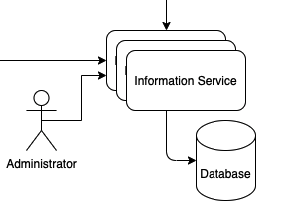
\includegraphics[scale=0.5]{figures/infobe}
			\fi
		\end{figure}
	\section{Administrator Panel}
		The administrator has special tools for maintaining the system and intervene in its internals, a special administrator panel that gives access to a 
		plethora of features that needs to be handled with care. 
		\begin{note}
			To connect to the administrator panel, we need to connect to the following addresses\\
			\begin{center}
				(if online) https://uortmc-infobe.herokuapp.com/admin/ \\
				(local machine )http://127.0.0.1:3001/admin
			\end{center}
			Please refer to the chapter \ref{cicd-versioning-deployment} and chapter \ref{start-stop-guide} for more details around how to connect.
		\end{note}
		\subsection{Admin Panel Login}
			\begin{figure}[H]
				\iftrue
				\caption{Administrator Panel}
				\centering
				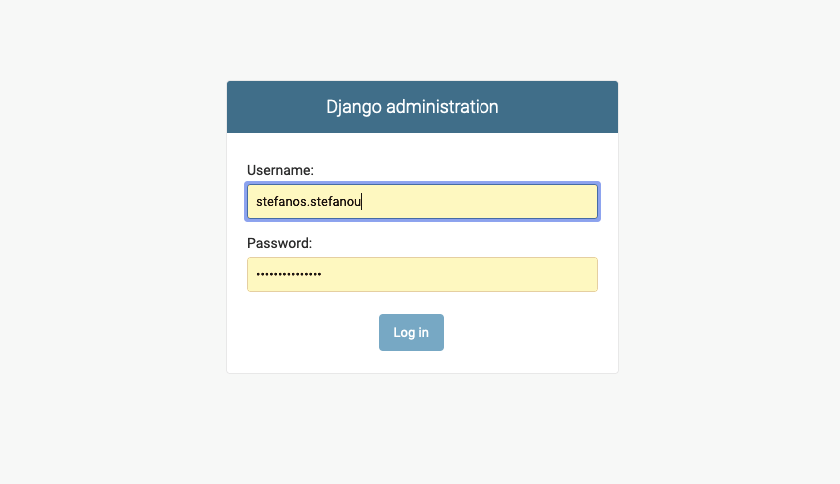
\includegraphics[scale=0.3]{figures/admin-panel-login}
				\fi
			\end{figure}
			The login screen is the first screen that an admin should encounter. The information transmitted into the Information Service
			is encrypted using HHTPS[\cite{rfc2818}] and transformed to an salted[\cite{MANBER1996171}] MD5 Hash[\cite{rfc1321}] for maximum 
			possible security.
		\subsection{Admin Panel Features}
			\begin{figure}[H]
				\iftrue
				\caption{Administrator Panel-Home}
				\centering
				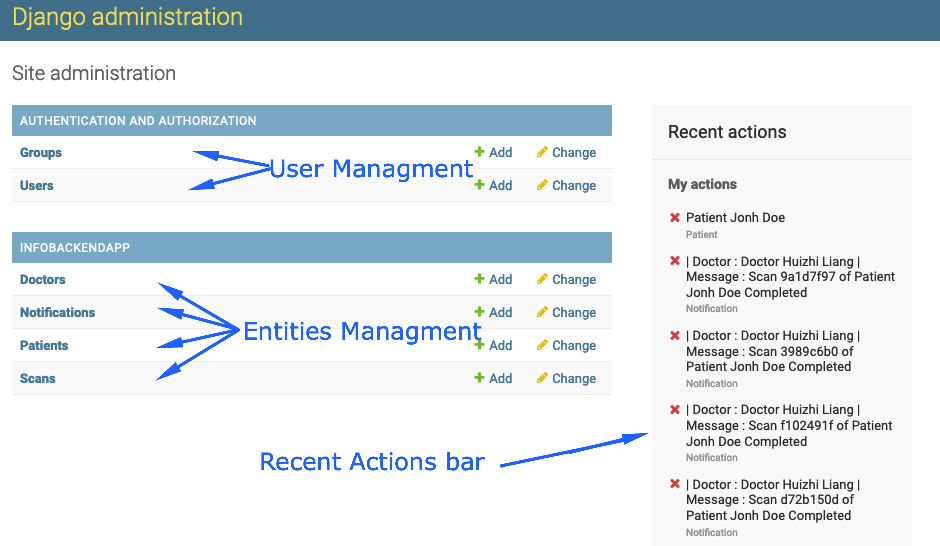
\includegraphics[scale=0.3]{figures/admin-panel-home}
				\fi
			\end{figure}
			After the login sequence is completed, the administrator will be redirected to the panel's home page; there, 
			it has available all the functionality needed to perform changes on the system. An administrator 
			has the right to alter the system's properties as well as the entity's attributes. We can add, alter and 
			delete entities at will, using the Entities Management.
			\begin{figure}[H]
				\iftrue
				\caption{Example deletion of a scan}
				\centering
				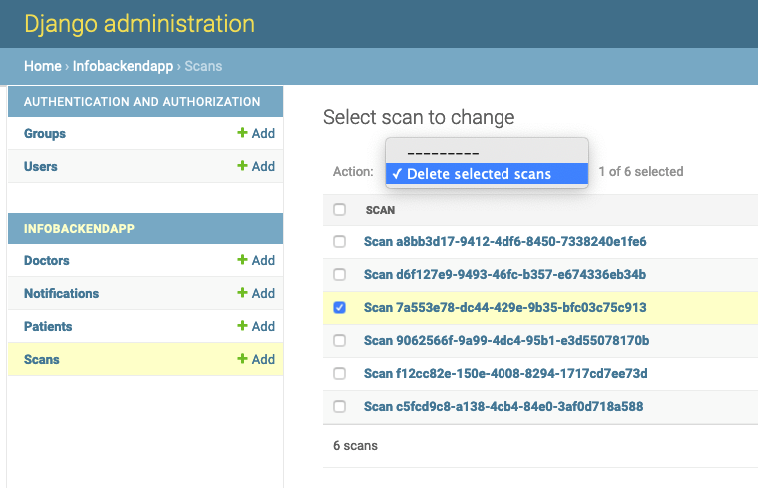
\includegraphics[scale=0.3]{figures/admin-panel-example-1}
				\fi
			\end{figure}
			\begin{figure}[H]
				\iftrue
				\caption{Example alteration of a patient}
				\centering
				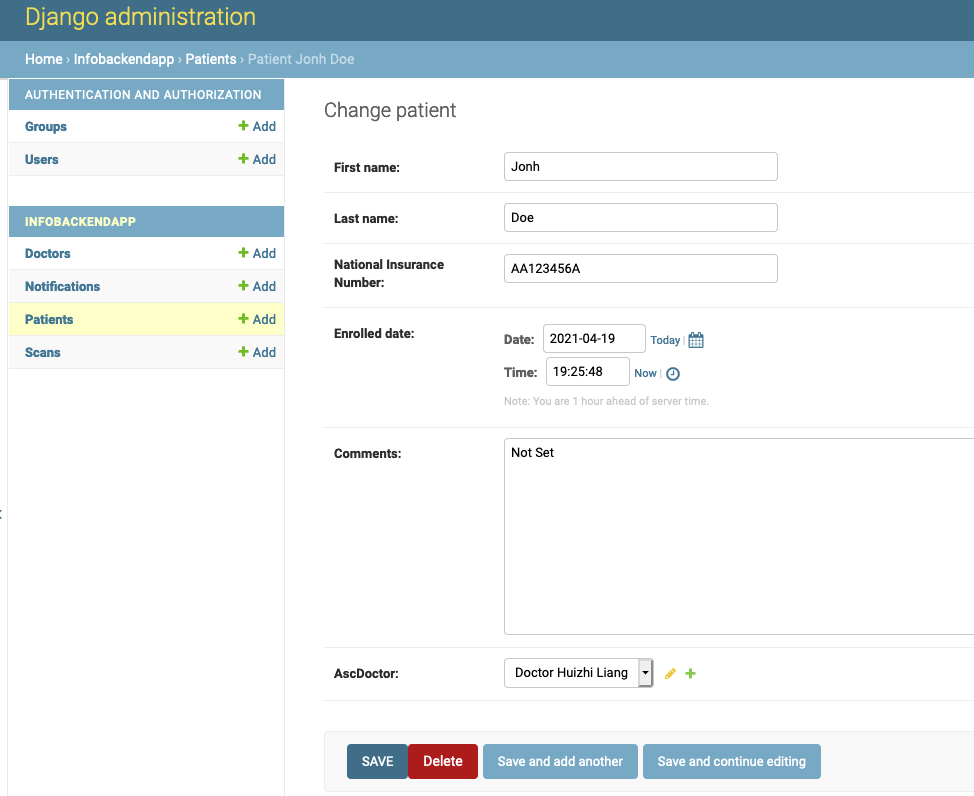
\includegraphics[scale=0.3]{figures/admin-panel-example-2}
				\fi
			\end{figure}
			
		
			
			
			
			
			
			
		
	



